% =============================================================================
\section{Nivel 2: decidir solo}
% =============================================================================

% ----------------------------------------------------------------------------- 4
\begin{frame}{Misión 4: la geocerca del concierto}
  \begin{columns}[c]
    \column{0.5\textwidth}
    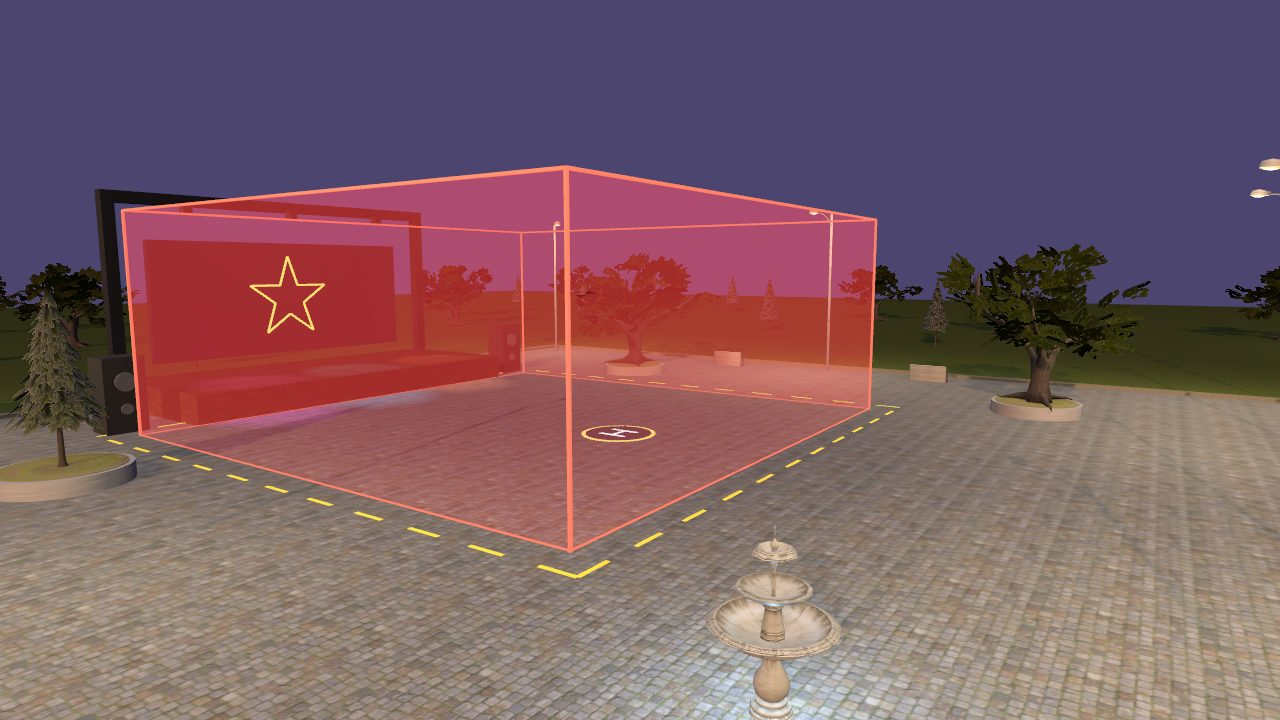
\includegraphics[width=\linewidth]{plaza_concierto}
    \column{0.47\textwidth}\small
    \textbf{Escenario}: en un concierto el dron no puede salirse de una caja de
    20\,$\times$\,20\,$\times$\,8 m.
    \begin{itemize}
      \item Un nodo \textbf{guardián} que \textbf{no vuela}: solo vigila.
      \item Si el dron va a salirse: \textbf{Hold}, y ya quieto, \textbf{Return}.
      \item Funciona \textbf{sin importar quién vuela}: un nodo, QGC o un piloto.
      \item \textbf{Viene de}: \cmd{flight\_mode\_monitor} + \cmd{return\_home}.
    \end{itemize}
  \end{columns}
\end{frame}

\begin{frame}{La caja}
  \begin{columns}[c]
    \column{0.47\textwidth}\centering
    \begin{tikzpicture}[scale=0.17]
      \draw[orange,dashed,thick] (-11,-7) rectangle (11,15);
      \draw[rojo,thick,fill=red!8] (-10,-6) rectangle (10,14);
      \fill[gray!40] (-8,14) rectangle (8,21);
      \node[font=\tiny] at (0,17.5) {escenario};
      \node[draw,circle,fill=azulclaro,inner sep=0.5pt,font=\tiny] at (0,0) {H};
      \draw[-{Stealth}] (0,0) -- (0,4) node[above,font=\tiny] {N};
      \node[font=\tiny,rojo] at (6,-4.5) {zona permitida};
      \node[font=\tiny,orange] at (6,-8.7) {límite +1 m};
    \end{tikzpicture}
    \column{0.5\textwidth}\small
    En NED desde el despegue (parámetros del nodo):
    \begin{center}
      \begin{tabular}{ll}
        \toprule
        norte & $-6 \ldots 14$ m \\
        este  & $-10 \ldots 10$ m \\
        altura & hasta 8 m \\
        \bottomrule
      \end{tabular}
    \end{center}
    Las paredes rojas son solo visuales: el dron las atraviesa. La \textbf{línea naranja punteada}
    del piso está 1 m afuera: es el criterio de éxito.
  \end{columns}
\end{frame}

\begin{frame}{¿Por qué no basta con revisar si ya se salió?}
  \begin{columns}[c]
    \column{0.52\textwidth}\small
    El dron \textbf{no frena en seco}. Desde que el guardián detecta hasta que el dron se detiene:
    \[ d = \underbrace{v\,t_r}_{\text{reacción}} + \underbrace{\frac{v^2}{2a}}_{\text{frenado}} \]
    Medido en SITL: a 4 m/s el x500 en Hold recorre todavía \textasciitilde4.5 m
    (frena a \textasciitilde2.4 m/s$^2$).
    \vspace{0.3em}
    \begin{idea}
      \small Hay que \textbf{predecir} dónde se va a detener y actuar si \emph{ese} punto queda fuera.
    \end{idea}
    \column{0.45\textwidth}
    \begin{tikzpicture}[x=0.5cm,y=0.5cm]
      \draw[rojo,thick] (8,-1) -- (8,3) node[above,font=\tiny] {cerca};
      \draw[orange,dashed] (9,-1) -- (9,3) node[above,font=\tiny] {+1 m};
      \fill[azul] (2,1) circle (4pt) node[below,font=\tiny] {ahora};
      \draw[-{Stealth},azul] (2,1) -- (3.6,1);
      \fill[gray] (5,1) circle (3pt) node[below,font=\tiny,align=center] {detenido\\(predicción)};
      \draw[decorate,decoration={brace,amplitude=4pt}] (2,1.6) -- (5,1.6) node[midway,above=3pt,font=\tiny] {$v t_r + v^2/2a$};
    \end{tikzpicture}
  \end{columns}
\end{frame}

\begin{frame}{Prueba de la fórmula}
  \small Frenando con aceleración constante $a$ desde $v$:
  \[ v(t) = v - a t \;\Rightarrow\; t_{\text{alto}} = \frac{v}{a}
     \qquad
     d = v\,t_{\text{alto}} - \tfrac12 a\,t_{\text{alto}}^2 = \frac{v^2}{a} - \frac{v^2}{2a} = \frac{v^2}{2a} \]
  \centering
  \begin{tabular}{rrr}
    \toprule
    $v$ (m/s) & $d$ con $a = 2$ m/s$^2$, $t_r = 0.5$ s & lo que hay que anticipar \\
    \midrule
    2 & $1.0 + 1.0 = 2.0$ m & poco \\
    4 & $2.0 + 4.0 = 6.0$ m & más que la tolerancia \\
    6 & $3.0 + 9.0 = 12.0$ m & más de la mitad de la caja \\
    \bottomrule
  \end{tabular}
  \vspace{0.4em}

  \raggedright\footnotesize Por eso \cmd{brake\_accel} = 2.0 y \cmd{reaction} = 0.5 por defecto: un poco más conservador que lo medido.
\end{frame}

\begin{frame}[fragile]{Tu parte en el guardián}
  \begin{lstlisting}[style=cpp,caption={guardian\_geocerca: los tres TODO}]
Vec3 stop_point() const {          // TODO 1: dónde se detendría
  // cada eje avanza  v * reaction_  +  v * |v| / (2 a)   (v*|v| conserva el signo)
}
case State::WATCH:                 // TODO 2: si stop_point() queda afuera
  // (outside_by(...) > 0): px4_.request_hold(), avisar y pasar a BRAKING
case State::BRAKING:               // TODO 3: casi quieto (speed() < 0.3) y en Hold:
  // px4_.return_home() y RETURNING. Si en 1 s no entró a Hold, pedirlo otra vez.
  \end{lstlisting}
  \small Ya hechos: \cmd{outside\_by(p)} (cuánto está afuera un punto), \cmd{speed()},
  \cmd{distance\_to\_edge()} y la medición de cuánto se salió.
\end{frame}

\begin{frame}[fragile]{Probarlo: el piloto travieso}
  \begin{lstlisting}[style=bash,caption={Tres terminales}]
vespo up --sim --world plaza_concierto
ros2 run x500_retos guardian_geocerca
ros2 run x500_retos vuelo_prueba --ros-args -p direction_deg:=0.0 -p speed:=6.0
  \end{lstlisting}
  \begin{columns}[c]
    \column{0.5\textwidth}\small
    \cmd{vuelo\_prueba} (ya completo) despega y se lanza en línea recta sin frenar, hasta que
    alguien le quite el control o llegue a \cmd{max\_distance} (30 m, red de seguridad).
    \vspace{0.3em}

    \cmd{direction\_deg}: 0 = norte (hay 14 m para acelerar), 90 = este, 180 = sur.
    \column{0.47\textwidth}
    \begin{terminal}{guardian\_geocerca}
¡Se va a salir! (a 5.1 m de la\\
\ orilla, va a 5.5 m/s): Hold\\
Detenido a 0.00 m fuera. Return\\
Lo más que se salió: 0.00 m OK
    \end{terminal}
  \end{columns}
\end{frame}

\begin{frame}{Un detalle de la vida real: Return se sale por arriba}
  \begin{columns}[c]
    \column{0.55\textwidth}\small
    Return sube primero a \cmd{RTL\_RETURN\_ALT} (30 m en el x500 de SITL, recortado por un cono
    cerca de casa). En la prueba subió a 9 m: \textbf{arriba de la caja}.
    \vspace{0.3em}

    El guardián no lo cuenta como falla suya (es configuración de PX4), pero avisa:
    \begin{terminal}{guardian\_geocerca}
Return subió a 9 m, arriba de la cerca:\\
\ baja RTL\_RETURN\_ALT en QGC
    \end{terminal}
    \column{0.42\textwidth}
    \begin{idea}
      \small En un concierto real eso se configura antes de volar: QGC $\rightarrow$ Parámetros
      $\rightarrow$ Return Mode, por debajo del techo de la geocerca.
    \end{idea}
  \end{columns}
\end{frame}

% ----------------------------------------------------------------------------- 5
\begin{frame}{Misión 5: cruzar una cueva}
  \begin{columns}[c]
    \column{0.5\textwidth}
    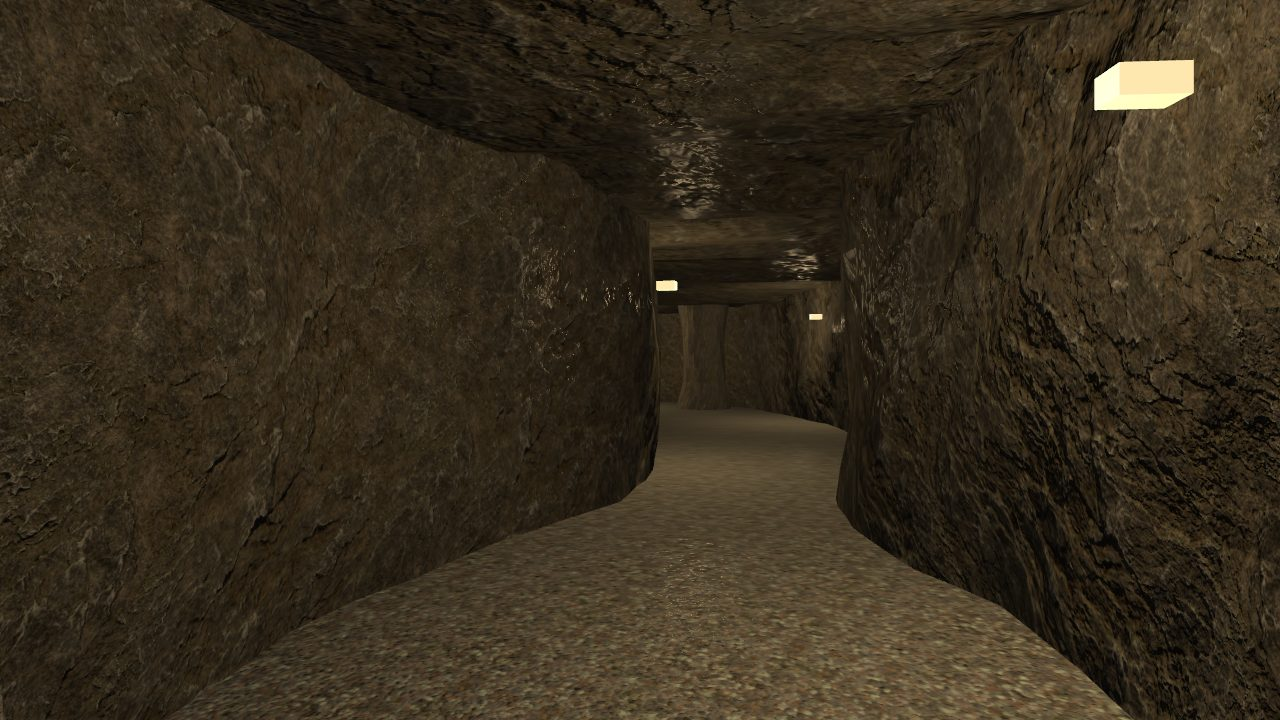
\includegraphics[width=\linewidth]{cueva_angostura}
    \column{0.47\textwidth}\small
    \textbf{Escenario}: atravesar un túnel curvo y oscuro usando \textbf{solo el lidar} para no chocar.
    \begin{itemize}
      \item Túnel de \textasciitilde66 m, 5 m de ancho, 4 m de alto.
      \item Dos angosturas de 3 m.
      \item Una columna de roca a medio camino: \textbf{solo se pasa por la izquierda}.
      \item \textbf{Viene de}: \cmd{velocity\_control}.
    \end{itemize}
  \end{columns}
\end{frame}

\begin{frame}{El mapa de la cueva}
  \centering
  \begin{tikzpicture}[x=0.12cm,y=0.09cm]
    \draw[gray!50,fill=gray!15] (-40,10) rectangle (40,76);
    \node[font=\tiny,gray] at (-28,70) {loma};
    \draw[azul,line width=3.5pt,opacity=0.5,smooth] plot coordinates {(0,10) (0,16) (2,23) (6,30) (8,37) (7,44) (3,50) (-1,56) (-3,63) (-2,70) (-1,76)};
    \draw[azul,thick,smooth] plot coordinates {(0,0) (0,10) (0,16) (2,23) (6,30) (8,37) (7,44) (3,50) (-1,56) (-3,63) (-2,70) (-1,76) (-1,84)};
    \node[draw,circle,fill=azulclaro,inner sep=0.5pt,font=\tiny] at (0,0) {H};
    \fill[orange] (-2.5,81.5) rectangle (0.5,86.5); \node[font=\tiny,right] at (1,84) {plataforma (N 84, E $-$1)};
    \fill[gray!70] (5.5,34) circle (1.5); \node[font=\tiny,right] at (9,34) {columna};
    \node[font=\tiny,right] at (4,23) {angostura};
    \node[font=\tiny,right] at (3,55) {angostura};
    \node[font=\tiny,right] at (1,11.5) {boca sur (N 10)};
    \node[font=\tiny,right] at (1,74.5) {boca norte (N 76)};
  \end{tikzpicture}
\end{frame}

\begin{frame}{El lidar 2D: \texttt{sensor\_msgs/LaserScan}}
  \begin{columns}[c]
    \column{0.45\textwidth}\centering
    \begin{tikzpicture}[scale=1]
      \fill[azul!10] (0,0) -- (-135+90:2) arc (-45:225:2) -- cycle;
      \foreach \a in {-120,-90,...,120} \draw[azul!40] (0,0) -- (\a+90:2);
      \draw[thick,fill=gray!30] (-0.25,-0.25) rectangle (0.25,0.25);
      \draw[-{Stealth},thick] (0,0.25) -- (0,0.9);
      \node[font=\tiny] at (0,2.25) {0° (frente)};
      \node[font=\tiny] at (-2.35,0) {+90° (izq)};
      \node[font=\tiny] at (2.35,0) {$-$90° (der)};
      \node[font=\tiny] at (0,-0.6) {$\pm$135° (atrás: ciego)};
    \end{tikzpicture}
    \column{0.52\textwidth}\small
    \begin{itemize}
      \item 1080 rayos de \cmd{angle\_min} $= -135^\circ$ a $+135^\circ$, cada \cmd{angle\_increment}.
      \item \cmd{ranges[i]}: distancia del rayo $i$ (m). \textbf{inf} si no pega en nada (hasta 30 m).
      \item Ángulo del rayo: \cmd{angle\_min + i * angle\_increment}.
      \item Ángulos \textbf{positivos a la izquierda} (FLU, convención de ROS).
      \item Va arriba del dron: el plano de escaneo está \textasciitilde0.3 m sobre el cuerpo.
    \end{itemize}
  \end{columns}
\end{frame}

\begin{frame}[fragile]{De Gazebo a ROS: el puente}
  \begin{lstlisting}[style=bash,caption={Lo que hace cueva.launch.py}]
ros2 run ros_gz_bridge parameter_bridge \
  /world/cueva/model/x500_lidar_2d_0/link/link/sensor/lidar_2d_v2/scan@sensor_msgs/msg/LaserScan[gz.msgs.LaserScan
#  ...y lo renombra a /x500/scan
  \end{lstlisting}
  \small
  \begin{itemize}
    \item \cmd{[} = solo de Gazebo hacia ROS. (\cmd{]} sería de ROS a Gazebo, \cmd{@} en ambos sentidos.)
    \item El nombre del topic de Gazebo incluye el mundo y el modelo (\cmd{x500\_lidar\_2d\_0}).
    \item \cmd{ros2 launch x500\_retos cueva.launch.py} levanta el puente y tu nodo juntos.
  \end{itemize}
\end{frame}

\begin{frame}{La herramienta: el mínimo de un sector}
  \begin{columns}[c]
    \column{0.45\textwidth}\centering
    \begin{tikzpicture}[scale=0.9]
      \fill[verde!25] (0,0) -- (75:2.2) arc (75:105:2.2) -- cycle;
      \fill[naranja!30] (0,0) -- (150:2.2) arc (150:210:2.2) -- cycle;
      \fill[naranja!30] (0,0) -- (-30:2.2) arc (-30:30:2.2) -- cycle;
      \draw[thick,fill=gray!30] (-0.2,-0.2) rectangle (0.2,0.2);
      \node[font=\tiny] at (90:2.5) {frente: $-15..15$};
      \node[font=\tiny] at (180:2.7) {izq: $60..120$};
      \node[font=\tiny] at (0:2.7) {der: $-120..-60$};
    \end{tikzpicture}
    \column{0.52\textwidth}\small
    Ya hecha en el nodo:
    \begin{center}\cmd{sector\_min(from\_deg, to\_deg)}\end{center}
    La distancia \textbf{más corta} que ve el lidar entre dos ángulos (positivo = izquierda). Lo que no
    pega en nada cuenta como \cmd{range\_max}.
    \vspace{0.3em}

    \footnotesize En el dibujo los sectores están girados: el frente va hacia arriba.
  \end{columns}
\end{frame}

\begin{frame}{Tu parte: \texttt{steer()}, del scan a una velocidad}
  \small Se llama 20 veces por segundo. Regresa \cmd{forward}, \cmd{left} (m/s) y \cmd{yawrate} (rad/s):
  \begin{enumerate}
    \item \textbf{Centrarse}: compara izquierda contra derecha y muévete hacia el lado con más espacio,
      proporcional a la diferencia y con tope. Afuera de la cueva un lado da 30 m: usa
      \cmd{std::min(d, 3.0)} para que solo cuenten las paredes cercanas.
    \item \textbf{Girar con la cueva}: busca el ángulo entre $-75^\circ$ y $75^\circ$ con más espacio libre y gira
      hacia él. Mejor: el espacio de cada ángulo como el \textbf{mínimo de una ventana} de $\pm10^\circ$,
      para no meterte por una rendija donde no cabes.
    \item \textbf{Avanzar}: más rápido si el frente está libre, más lento si hay que girar mucho.
  \end{enumerate}
  \begin{idea}
    \small Ya hecho: si hay algo a menos de \cmd{stop\_distance} al frente, no avanza; si pasa
    \cmd{stuck\_time} sin moverse, aterriza ``atorado''.
  \end{idea}
\end{frame}

\begin{frame}{Buscar el hueco: ventanas, no rayos}
  \begin{columns}[c]
    \column{0.5\textwidth}\centering
    \begin{tikzpicture}[scale=0.8]
      \draw[thick] (-2.5,3) -- (-0.15,3); \draw[thick] (0.15,3) -- (2.5,3);
      \draw[thick] (-2.5,3) -- (-2.5,-0.3); \draw[thick] (2.5,3) -- (2.5,-0.3);
      \fill[gray!60] (1.2,1.8) circle (0.5);
      \draw[rojo,thick] (0,0) -- (0,3.6) node[above,font=\tiny,align=center] {un rayo largo\\por la rendija};
      \fill[verde!30,opacity=0.6] (0,0) -- (-1.5,3) -- (-0.4,3) -- cycle;
      \node[font=\tiny,verde!50!black] at (-1.6,1.2) {ventana libre};
      \draw[thick,fill=azulclaro] (-0.2,-0.2) rectangle (0.2,0.2);
    \end{tikzpicture}
    \column{0.47\textwidth}\small
    Un solo rayo puede ``ver'' muy lejos por una rendija de 20 cm donde el x500 (\textasciitilde0.75 m de
    punta a punta) no cabe.
    \vspace{0.3em}

    Tomar el \textbf{mínimo} de una ventana de $\pm10^\circ$ es pedir que \emph{todo} ese cono esté libre.
  \end{columns}
\end{frame}

\begin{frame}{FLU contra NED: los signos}
  \small \cmd{steer()} piensa como el lidar (FLU: izquierda y giro a la izquierda positivos). El nodo ya
  convierte al mandar a PX4:
  \[
    \begin{aligned}
      v_N &= f\cos\psi + l\sin\psi \\
      v_E &= f\sin\psi - l\cos\psi \\
      \dot\psi_{\text{NED}} &= -\,\text{yawrate}
    \end{aligned}
  \]
  \begin{columns}[c]
    \column{0.5\textwidth}
    \begin{itemize}
      \item $f$ = adelante, $l$ = izquierda, $\psi$ = heading.
      \item Con $\psi = 0$ (al norte): izquierda = oeste $\Rightarrow v_E = -l$ \ok.
    \end{itemize}
    \column{0.47\textwidth}
    \begin{idea}
      \small La altura va fija por posición (\cmd{z} = $-1.5$) y lo horizontal por velocidad: un
      \textbf{setpoint mixto}.
    \end{idea}
  \end{columns}
\end{frame}

\begin{frame}{Flujo y calificación de la cueva}
  \begin{columns}[c]
    \column{0.45\textwidth}
    \begin{tikzpicture}[node distance=0.25cm,st/.style={draw=azul,fill=azulclaro,rounded corners,font=\tiny,minimum width=2.2cm}]
      \node[st] (a) {WARMUP / TAKEOFF};
      \node[st,below=of a] (b) {TO\_ENTRANCE (posición)};
      \node[st,below=of b,fill=yellow!20] (c) {CAVE (lidar)};
      \node[st,below=of c] (d) {TO\_PAD (posición)};
      \node[st,below=of d] (e) {LANDING};
      \draw[-{Stealth}] (a)--(b); \draw[-{Stealth}] (b)--node[right,font=\tiny]{1 m adentro de la boca}(c);
      \draw[-{Stealth}] (c)--node[right,font=\tiny]{norte \textgreater 78 m}(d); \draw[-{Stealth}] (d)--(e);
    \end{tikzpicture}
    \column{0.52\textwidth}\small
    \textbf{¿Por qué entrar por posición?} Afuera, el rayo más largo no apunta a la boca: apunta al
    vacío de los lados.
    \begin{terminal}{al aterrizar}
cruzó la cueva: sí OK\\
del lidar a la roca, mínimo:\\
\ \ 1.16 m (límite 0.6) OK\\
a 0.16 m de la plataforma OK\\
Misión cumplida
    \end{terminal}
  \end{columns}
\end{frame}
